\chapter{Mathematical Background}
\label{sec:mb}

This chapter establishes the mathematical foundations necessary for modern cryptography. The concepts introduced here --- probabilistic polynomial-time adversaries, negligible probabilities, and computational hardness assumptions --- form the bedrock upon which all cryptographic security definitions rest. Understanding these foundations is crucial because they allow us to formalize what it means for a cryptographic scheme to be "secure" in a way that is both mathematically rigorous and practically meaningful.

In modern cryptography, (1) we typically assume that our attackers cannot run in unreasonably large amounts of time, and (2) we allow security to be broken with a \emph{very small}, but non-zero, probability.
Without these assumptions, we must work in the realm of information-theoretic cryptography, which is often unachievable or impractical for many applications. For example, the one-time pad\footnote{For a message $m \in \{0,1\}^n$ and a random key $k \in \{0,1\}^n$, the encryption of $m$ is $c = m \oplus k$. The decryption is $m = c \oplus k$.}
--- an information-theoretically secure cipher --- is not very useful because it requires very large keys.

Below, we define items (1) and (2) more formally. We require our adversaries to run in polynomial time, which captures the idea that their runtime is not unreasonably large (sections~\ref{ssec:ppt}). We also allow security to be broken with very small, or negligible, probability (section ~\ref{ssec:nnf}). 

\section{Probabilistic Polynomial Time}
\label{ssec:ppt}
A probabilistic Turing Machine is a generic computer that is allowed to make random choices during its execution. This randomness is essential in cryptography: adversaries may use randomness in their attacks, and cryptographic algorithms themselves require randomness for security. A probabilistic \textit{polynomial time} Turing Machine is one which halts in time polynomial in its input length. Note that any deterministic polynomial-time algorithm is trivially a PPT algorithm (it simply ignores its random tape), but the converse is not necessarily true---probabilistic algorithms can sometimes solve problems more efficiently than deterministic ones. More formally:

\begin{definition}[Probabilistic Polynomial Time]
A probabilistic Turing Machine $M$ is said to be PPT (a Probabilistic Polynomial Time Turing Machine) if $\exists c \in \mathbb{Z}^+$ such that $\forall x \in\{0,1\}^*$, $M(x)$ halts in $|x|^c$ steps.
\end{definition}

A {\em non-uniform} PPT Turing Machine is a collection of machines one for each input length, as opposed to a single machine that must work for all input lengths. Non-uniformity allows each machine $M_n$ to have "advice" specific to inputs of length $n$, which can be thought of as a polynomial-sized lookup table. This models adversaries who may have precomputed information or special knowledge about specific input lengths. While non-uniform PPT is a stronger model than uniform PPT (any uniform PPT algorithm is also non-uniform PPT), it is often more convenient for security reductions and captures realistic adversarial capabilities.

\begin{definition}[Non-uniform PPT]
A non-uniform PPT machine is a sequence of Turing Machines $\{ M_1, M_2, \cdots \}$ such that $\exists c \in \mathbb{Z}^+$ such that $\forall x \in\{0,1\}^*$, $|M_{|x|} |$ if of size $\leq |x|^c$ and $M_{|x|}(x)$ halts in $|x|^c$ steps.
\end{definition}



\section{Noticeable and Negligible Functions}
\label{ssec:nnf}
Noticeable and negligible functions are used to characterize the ``largeness'' or ``smallness'' of a function describing the probability of some event.  Intuitively, a noticeable function is required to be larger than some inverse-polynomially function in the input parameter. On the other hand, a negligible function must be smaller than any inverse-polynomial function of the input parameter. More formally:


\begin{definition}[Noticeable Function]
A function $\mu(\cdot): \mathbb{Z}^+ \rightarrow [0,1]$ is noticeable iff $\exists c \in \mathbb{Z}^+, n_0 \in \mathbb{Z}^+$ such that $\forall n \geq n_0 , \; \mu(n) > n^{-c}$.
\end{definition}

\paragraph{Example.} Observe that $\mu(n) = n^{-3}$ is a noticeable function.  (Notice that the above definition is satisfied for $c = 4$ and $n_0 = 1$.)

\begin{definition}[Negligible Function]
A function $\mu(\cdot): \mathbb{Z}^+ \rightarrow [0,1]$ is negligible iff $\forall c \in \mathbb{Z}^+ \; \exists n_0 \in \mathbb{Z}^+$ such that $\forall n \geq n_0 , \; \mu(n) < n^{-c}$.
\end{definition}

\paragraph{Example.} $\mu(n) = 2^{-n}$ is an example of a negligible function. This can be observed as follows.
Consider an arbitrary $c \in \mathbb{Z}^+$ and set $n_0 = c^2$. We will show that for all $n \geq n_0$, we have $\mu(n) = 2^{-n} < n^{-c}$.

First, we establish that $2^{-n} = n^{-\frac{n}{\log_2 n}}$. This follows from taking logarithms: 
$$\log_2(2^{-n}) = -n = \log_2(n^{-\frac{n}{\log_2 n}}) = -\frac{n}{\log_2 n} \cdot \log_2 n = -n.$$

Now, we need to show that for $n \geq n_0 = c^2$, we have $\frac{n}{\log_2 n} \geq c$. Since the function $f(n) = \frac{n}{\log_2 n}$ is increasing for $n \geq e$, it suffices to show that $f(c^2) \geq c$. We have:
$$f(c^2) = \frac{c^2}{\log_2(c^2)} = \frac{c^2}{2\log_2 c} = \frac{c}{2} \cdot \frac{c}{\log_2 c}.$$

For $c \geq 4$, we have $\frac{c}{\log_2 c} \geq 2$ (since $4/\log_2 4 = 2$ and the function $c/\log_2 c$ is increasing for $c \geq e$), so $f(c^2) \geq \frac{c}{2} \cdot 2 = c$. For $c \in \{1,2,3\}$, we can verify directly: $f(1) = 0$, $f(4) = 2$, $f(9) \approx 2.85$, so we may need to choose a larger $n_0$ for small $c$. However, since we only need existence of some $n_0$, we can set $n_0 = \max(c^2, 16)$ for $c \leq 3$, and then $f(n_0) \geq f(16) = 4 \geq c$.

Therefore, for $n \geq n_0$, we have $\frac{n}{\log_2 n} \geq c$, which implies $-\frac{n}{\log_2 n} \leq -c$. Since $n > 1$, this gives us:
$$\mu(n) = 2^{-n} = n^{-\frac{n}{\log_2 n}} \leq n^{-c}.$$

Thus, we have proved that for any $c \in \mathbb{Z}^+$, there exists $n_0 \in \mathbb{Z}^+$ such that for any $n \geq n_0$, $\mu(n) < n^{-c}$.

\paragraph{Gap between Noticeable and Negligible Functions.}
At first thought it might seem that a function that is {not} negligible (or, a non-negligible function) must be a noticeable. This is not true!\cite{JC:Bellare02} Negating the definition of a negligible function, we obtain that a non-negligible function $\mu(\cdot)$ is such that $\exists c \in \mathbb{Z}^+$ such that $\forall n_0 \in \mathbb{Z}^+$, $\exists n \geq n_0$ such that $\mu(n) > n^{-c}$.
Note that this requirement is satisfied as long as $\mu(n) > n^{-c}$ for infinitely many choices of $n \in \mathbb{Z}^+$. However, a noticeable function requires this condition to be true for every $n \geq n_0$.

Below we give example of a function $\mu(\cdot)$ that is neither negligible nor noticeable.
$$\mu(n) = \Big\{
\begin{array}{ll}
  2^{-n} & : n \mod 2 = 0\\
  n^{-3} & : n \mod 2 \neq 0
\end{array}
$$
This function is obtained by interleaving negligible and  noticeable functions. For even $n$, $\mu(n) = 2^{-n}$ which is negligible. For odd $n$, $\mu(n) = n^{-3}$ which is noticeable. Specifically, it's not negligible because $\mu(n) = n^{-3} > n^{-4}$ for all odd $n$, violating the definition. It's not noticeable because $\mu(n) = 2^{-n} < n^{-c}$ for any fixed $c$ and all sufficiently large even $n$, so there's no $n_0$ such that $\mu(n) > n^{-c}$ for all $n \geq n_0$.

\paragraph{Properties of Negligible Functions.} Sum and product of two negligible functions is still a negligible function. We argue this for the sum function below and defer the problem for products to Exercise~\ref{ex:product}. These properties together imply that any polynomial function of a negligible function is still negligible.

\paragraph{Practical Intuition.} To build intuition, consider that a negligible probability means the event is so rare it's essentially impossible in practice. For example, if a cryptographic scheme has a negligible probability $\mu(n) = 2^{-128}$ of being broken, this is smaller than the probability of being struck by lightning twice in one's lifetime (approximately $10^{-12}$). Even for $n = 64$, we have $2^{-64} \approx 5 \times 10^{-20}$, which is astronomically small. This is why we can safely ignore negligible probabilities when reasoning about cryptographic security.

\begin{exercise}\label{ex:product}
If $\mu(n)$ and $\nu(n)$ are negligible functions from domain $\mathbb{Z}^+$ to range $[0,1]$ then prove that the following functions are also negligible functions:
\begin{enumerate}
    \item $\psi_1(n) = \frac{1}{2} \cdot \left(\mu(n) + \nu(n)\right)$
    \item $\psi_2(n) = \min\{\mu(n) + \nu(n), 1\}$
    \item $\psi_3(n) = \mu(n)\cdot \nu(n)$
    \item $\psi_4(n) = \mathsf{poly}(\mu(n))$, where $\mathsf{poly}(\cdot)$ is an unspecified polynomial function. (Assume that the output is also clamped to $[0,1]$ to satisfy the definition)
\end{enumerate}
\end{exercise}
\proof 
$ $
\begin{enumerate}
    \item We need to show that for any $c \in \mathbb{Z}^+$, we can find $n_0$ such that $\forall n \geq n_0$, $\psi_1(n) \leq n^{-c}$. Our argument proceeds as follows. Given the fact that $\mu$ and $\nu$ are negligible we can conclude that there exist $n_1$ and $n_2$ such that $\forall n \geq n_1$, $\mu(n) < n^{-c}$ and $\forall n \geq n_2$, $\nu(n) < n^{-c}$. Combining the above two facts and setting $n_0 = \max(n_1, n_2)$ we have that for every $n \geq n_0$,
    \begin{align*}
        \psi_1(n) &= \frac{1}{2} \cdot (\mu(n) + \nu(n)) < \frac{1}{2} \cdot (n^{-c} + n^{-c}) = n^{-c}
    \end{align*}
    Thus, $\psi_1(n) \leq n^{-c}$ and hence is negligible.

    \item We need to show that for any $c \in \mathbb{Z}^+$, we can find $n_0$ such that $\forall n \geq n_0$, $\psi_2(n) \leq n^{-c}$. Given the fact that $\mu$ and $\nu$ are negligible, there exist $n_1$ and $n_2$ such that $\forall n \geq n_1$, $\mu(n) \leq n^{-c-1}$ and $\forall n \geq n_2$, $\nu(n) \leq n^{-c-1}$. Setting $n_0 = \max(n_1, n_2, 3)$ we have that for every $n \geq n_0$,
    \begin{align*}
        \psi_2(n) &= \min\{\mu(n) + \nu(n), 1\} < n^{-c-1} + n^{-c-1} = 2n^{-c-1} = 2n^{-1} \cdot n^{-c} \leq n^{-c}
    \end{align*}
    since $n \geq 3$ implies $2n^{-1} \leq 1$.
    \item The proof that $\psi_3(n) = \mu(n) \cdot \nu(n)$ is negligible follows similarly: since both $\mu(n)$ and $\nu(n)$ are less than $n^{-c}$ for sufficiently large $n$, their product is less than $n^{-2c} < n^{-c}$.
    
    \item For $\psi_4(n) = \mathsf{poly}(\mu(n))$, since $\mu(n)$ is negligible, we have $\mu(n) < n^{-c}$ for any $c$ and sufficiently large $n$. If $\mathsf{poly}$ is a polynomial of degree $d$, then $\mathsf{poly}(\mu(n)) < \mathsf{poly}(n^{-c}) = O(n^{-cd})$, which is still negligible. The details are left as an exercise.
\end{enumerate}
\qed

%\begin{corollary}
%If $f(n)$ is non-negligible and $g(n)$ is negligible, then $h(n) = f(n) - g(n)$ is non-negligible.
%\end{corollary}
%
%\proof If $h(n)$ was negligible, then $f(n) = g(n) + h(n)$ would be the sum of two negligible functions, but would be non-negligible, which is a contradiction.  \qed

\section{Computationally  Hard Problems}\label{sec:assumptions}
%So far, much of our investigation relied on the existence of one-way-functions or in certain cases on the existence of one-one one-way functions. However, just the mere existence of an object is not enough for real-world implementations. 
We will next provide certain number theoretical problems that are conjectured to be computationally intractable. We will use the conjectured hardness of these problems in subsequent chapters to provide concrete instantiations. These assumptions---discrete logarithm, Diffie-Hellman, and factoring---form the foundation for most practical public-key cryptography. They have been studied for decades and are widely believed to be hard, though proving their hardness would resolve major open problems in complexity theory (such as showing $P \neq NP$).

\subsection{The Discrete-Log Family of Problem}
Consider a group $\mathbb{G}$ of prime order. For example, consider the group $\mathbb{Z}_p^*$ where $p$ is a large prime. Let $g$ be a generator of this group $\mathbb{G}$. In this group, given $g^x$ for a random $x \in \{1,\ldots p-1\}$ consider the problem of finding $x$. This problem, referred to as the discrete-log problem, is believed to be computationally hard.

The asymptotic definition of the discrete-log problem needs to consider an infinite family of groups or what we will a group ensemble. 

\paragraph{Group Ensemble.} A group ensemble is a set of finite cyclic groups $\mathcal{G} =\{ \mathbb{G}_n\}_{n \in \mathbb{N}}$. For the group $G_n$, we assume that given two group elements in $G_n$, their group operation (which we denote additively or multiplicatively depending on context)    can be computed in polynomial in $n$ time. Additionally, we assume that given $n$ the generator $g$ of $\mathbb{G}_n$ can be computed in polynomial time. 

\begin{definition}[Discrete-Log Assumption]\label{def:dl}
We say that the discrete-log assumption holds for the group ensemble $\mathcal{G} =\{ \mathbb{G}_n\}_{n \in \mathbb{N}}$, if for every non-uniform PPT algorithm $\mathcal{A}$ we have that
\[\mu_\mathcal{A}(n) := \Pr_{x \leftarrow |G_n|}[\mathcal{A}(g,g^x) = x]\]
is a negligible function.
\end{definition}

\paragraph{The Diffie-Hellman Problems.} In addition to the discrete-log assumption, we also define the Computational Diffie-Hellman Assumption and the Decisional Diffie-Hellman Assumption. 
\begin{marginfigure}
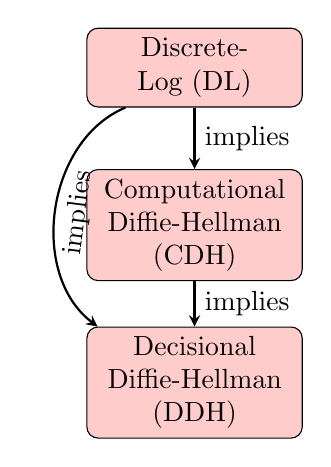
\begin{tikzpicture}[
    node distance=2cm,
    assumption/.style={rectangle, draw, fill=red!20, text width=2.5cm, text centered, rounded corners, minimum height=1cm},
    arrow/.style={->, >=stealth, thick}
]
\node[assumption] (dl) {Discrete-Log (DL)};
\node[assumption, below of=dl] (cdh) {Computational Diffie-Hellman (CDH)};
\node[assumption, below of=cdh] (ddh) {Decisional Diffie-Hellman (DDH)};

\draw[arrow] (dl) -- node[right] {implies} (cdh);
\draw[arrow] (cdh) -- node[right] {implies} (ddh);
\draw[arrow, bend right=60] (dl) to node[below, sloped] {implies} (ddh);
\end{tikzpicture}
\caption{Relationship between discrete-log assumptions. DL is the weakest assumption; breaking DL allows breaking CDH, and breaking CDH allows breaking DDH. The reverse implications are not known to hold.}
\label{fig:assumptions}
\end{marginfigure}


\begin{definition}[Computational Diffie-Hellman (CDH) Assumption]\label{def:cdh}
We say that the Computational Diffie-Hellman Assumption holds for the group ensemble $\mathcal{G} =\{ \mathbb{G}_n\}_{n \in \mathbb{N}}$, if for every non-uniform PPT algorithm $\mathcal{A}$ we have that
\[\mu_\mathcal{A}(n) := \Pr_{x,y \leftarrow |G_n|}[\mathcal{A}(g,g^x,g^y) = g^{xy}]\]
is a negligible function.
\end{definition}

\begin{definition}[Decisional Diffie-Hellman (DDH) Assumption]\label{def:ddh}
We say that the Decisional Diffie-Hellman Assumption holds for the group ensemble $\mathcal{G} =\{ \mathbb{G}_n\}_{n \in \mathbb{N}}$, if for every non-uniform PPT algorithm $\mathcal{A}$ we have that
\[\mu_\mathcal{A}(n) = \mid\Pr_{x,y \leftarrow |G_n|}[\mathcal{A}(g,g^x,g^y,g^{xy}) = 1] - \Pr_{x,y,z \leftarrow |G_n|}[\mathcal{A}(g,g^x,g^y,g^{z}) = 1]\mid\]
is a negligible function.
\end{definition}

It is not hard to observe that the discrete-log assumption is the weakest of the three assumptions above. In fact, it is not difficult to show that the Discrete-Log Assumption for $\mathcal{G}$ implies the CDH and the DDH Assumptions for $\mathcal{G}$.  Additionally, we leave it as an exercise to show that the CDH Assumption for $\mathcal{G}$ implies the  DDH Assumptions for $\mathcal{G}$. Figure~\ref{fig:assumptions} illustrates the relationship between these assumptions.

\paragraph{Examples of Groups where these assumptions hold.} Now we provide some examples of group where these assumptions hold. 
\begin{enumerate}
    \item Consider the group $\mathbb{Z}_p^*$ for a prime $p$.\footnote{Since the number of primes is infinite we can define an infinite family of such groups. For the sake of simplicity, here we only consider a single group.} For this group the CDH Assumption is conjectured to be true. 
    
    However, 
    the DDH Assumption in this group can be shown to be false. Can you show how?
    

    \paragraph{Legendre Symbol.} Let $p$ be an odd prime number. An integer $a$ is said to be a \emph{quadratic residue} modulo $p$ if it is congruent to a perfect square modulo $p$ and is said to be a \emph{quadratic non-residue} modulo $p$ otherwise. The \emph{Legendre symbol} is a function of $a$ and $p$ defined as
    \begin{equation*}
        \left(\frac{a}{p}\right) = \begin{cases}
    1 &\text{if $a$ is quadratic residue mod $p$ and $a \not\equiv 0 \mod p$}\\
    -1 &\text{if $a$ is quadratic non-residue mod $p$}\\
    0 &\text{if $a \equiv 0 \mod p$}
    \end{cases}
    \end{equation*}
    The Legendre symbol can be efficiently computed as $\left(\frac{a}{p}\right) = a^{\frac{p-1}{2}}\mod p$.

    \paragraph{DDH is easy in this group.} This is because given $g^x, g^y$ one can easily compute deduce the Legendre symbol of $g^{xy}$.  Observe that if $\left(\frac{g}{p}\right) = -1$ then we have that $\left(\frac{g^{xy}}{p}\right) = 1$ if and only if $ \left(\frac{g^x}{p}\right) =1 $ or $\left(\frac{g^y}{p}\right) = 1$. Using this fact, we can construct an adversary that breaks the DDH problem with a non-negligible (in fact, noticeable) probability.

    \paragraph{Deployment.} The group $\mathbb{Z}_p^*$ has been widely deployed in classical cryptographic protocols, including the original Diffie-Hellman key exchange, ElGamal encryption, and the Digital Signature Algorithm (DSA). However, due to the weakness of the DDH assumption in this group, modern protocols typically use subgroups of prime order or elliptic curve groups instead. The group $\mathbb{Z}_p^*$ remains relevant for protocols that only require CDH security, such as some variants of ElGamal encryption.

    \item Let $p = 2q+1$ where both $p$ and $q$ are prime.\footnote{By Dirichet's Theorem on primes in arithmetic progression, we have that there are infinite choices of primes $(p,q)$ for which $p = 2q+1$. This allows us to generalize this group to a group ensemble.} Next, let $\mathbb{Q}$ be the order-$q$ subgroup of quadratic residues in $\mathbb{Z}^*_p$. For this group, the DDH assumption is believed to hold.

    
    \paragraph{Deployment.} The order-$q$ subgroup of quadratic residues in $\mathbb{Z}^*_p$ (where $p = 2q+1$ is a safe prime) has been used in various cryptographic protocols, including some implementations of the Diffie-Hellman key exchange and ElGamal encryption that require DDH security. However, these groups require larger key sizes (typically 2048-4096 bits) to achieve security levels comparable to elliptic curves, making them less efficient than modern elliptic curve alternatives. They are still used in some legacy systems and standards, but elliptic curve groups are generally preferred for new deployments due to their efficiency advantages.
    \item Let $N = pq$ where $p,q, \frac{p-1}{2}$ and $\frac{q-1}{2}$ are primes. Let $\mathbb{QR}_N$ be the cyclic subgroup of quadratic residues of order $\phi(N) = (p-1)(q-1)$. For this group $\mathbb{QR}_N$, the DDH assumption is also believed to hold.
    
    \paragraph{Deployment.} The group $\mathbb{QR}_N$ is closely related to RSA, which operates in $\mathbb{Z}_N^*$ (where $N = pq$). While standard RSA encryption and decryption work in the full group $\mathbb{Z}_N^*$ rather than specifically in $\mathbb{QR}_N$, the quadratic residues play an important role in RSA's security analysis and some variants. The group $\mathbb{QR}_N$ has been used in cryptographic constructions that require both DDH security and a connection to the factoring problem (as we will see, CDH in $\mathbb{QR}_N$ implies factoring). However, for discrete-log-based protocols, this group is less commonly deployed in practice compared to elliptic curve groups or safe prime subgroups, as it requires composite moduli and the security depends on both the discrete logarithm and factoring assumptions. It appears primarily in advanced cryptographic constructions and security reductions.
    \item Elliptic Curve groups: An elliptic curve over a finite field $\mathbb{F}_p$ is defined by an equation of the form $y^2 = x^3 + ax + b$ (for Weierstrass form) or $y^2 = x^3 + ax^2 + x$ (for Montgomery form), where $a, b \in \mathbb{F}_p$ and the curve is non-singular. The set of points $(x,y) \in \mathbb{F}_p \times \mathbb{F}_p$ satisfying the curve equation, together with a special "point at infinity" $\mathcal{O}$, forms an abelian group under a geometric addition operation. For cryptographic applications, we typically work with a cyclic subgroup of prime order $q$ of the elliptic curve group. The discrete-log, CDH, and DDH assumptions are all believed to hold for well-chosen elliptic curve groups.\footnote{There are infinitely many elliptic curves over various finite fields, allowing us to define group ensembles. The security of elliptic curve cryptography relies on the hardness of the elliptic curve discrete logarithm problem (ECDLP), which is believed to be exponentially harder than the discrete logarithm problem in finite fields of similar size.}
    
    \paragraph{secp256k1.} The secp256k1 curve is a Koblitz curve (a special type of elliptic curve) defined by the equation $y^2 = x^3 + 7$ over the prime field $\mathbb{F}_p$ where $p = 2^{256} - 2^{32} - 2^9 - 2^8 - 2^7 - 2^6 - 2^4 - 1$. It has prime order and provides approximately 128 bits of security. secp256k1 is most notably used in Bitcoin and Ethereum for ECDSA signatures, making it one of the most widely deployed elliptic curves in terms of economic value. Unlike Curve25519, secp256k1 uses the Weierstrass form, and its parameters were standardized by the Standards for Efficient Cryptography Group (SECG). 

    \paragraph{Curve25519.} Curve25519 is a widely-used elliptic curve designed by Daniel J. Bernstein in 2005. It is a Montgomery curve defined by the equation $y^2 = x^3 + 486662x^2 + x$ over the prime field $\mathbb{F}_p$ where $p = 2^{255} - 19$. The curve has prime order $q = 2^{252} + 27742317777372353535851937790883648493$, providing approximately 128 bits of security. The base point (generator) has $x$-coordinate $x = 9$. Curve25519 offers several advantages: (1) it enables fast, constant-time implementations that resist side-channel attacks, (2) it provides strong security with relatively small key sizes (256 bits), and (3) its parameters were chosen transparently for mathematical simplicity, avoiding concerns about hidden backdoors. Curve25519 is widely deployed in modern cryptographic protocols, including the Ed25519 signature scheme and the X25519 key exchange protocol.

\end{enumerate}

\paragraph{Is DDH strictly stronger than Discrete-Log?} In the example cases above, where DDH is known believed to be hard, the
best known algorithms for DDH are no better than the best known algorithms for the discrete-log problem. Whether the DDH assumption is strictly stronger than the discrete-log assumption is an open problem. 



\subsection{CDH in $\mathbb{QR}_N$ implies Factoring}

In this section, we will show that the CDH assumption in $\mathbb{QR}_N$ implies the factoring assumption. 
\begin{lemma}
Given an algorithm $\mathcal{A}$ that breaks the CDH assumption in $\mathbb{QR}_N$, we construct an non-uniform PPT adversary $\mathcal{B}$ that on input $N$ outputs its prime factors $p$ and $q$.
\end{lemma}
\begin{proof}
Given that $\mathcal{A}$ is an algorithm that solves the CDH problem in $\mathbb{QR}_N$ with a non-negligible probability, we construct an algorithm $\mathcal{B}$ that can factor $N$. The reduction works by using $\mathcal{A}$ to find square roots that help factor $N$. Specifically, $\mathcal{B}$ on input $N$ proceeds as follows:
\begin{enumerate}
\item Sample a random value $r$ in $\mathbb{Z}_N^*$ and compute $v := r^2 \mod N$. Note that $v \in \mathbb{QR}_N$. Then compute $g := v^2 \mod N$. Note that $g$ is a generator of $\mathbb{QR}_N$ with high probability, since $v$ is a random quadratic residue and squaring preserves the cyclic structure.
\item Sample $x, y \leftarrow [N]$.\footnote{Note that sampling $x,y$ uniformly from $[N]$ is statistically close to sampling $x,y$ uniformly from $[\phi(N)]$.} The statistical closeness follows from the fact that $N$ and $\phi(N) = (p-1)(q-1)$ are relatively close: $|N - \phi(N)| = p + q - 1 = O(\sqrt{N})$, so the statistical distance is $O(1/\sqrt{N})$, which is negligible.
\item Let $ u := \mathcal{A}(g, g^{x}\cdot v, g^y\cdot v)$\footnote{Note that $g^x\cdot v$ where $x \leftarrow [N]$ is statistically close to $g^x$ where $x \leftarrow [N]$.} The inputs $g^x \cdot v$ and $g^y \cdot v$ are constructed to "hide" the actual CDH inputs while still allowing $\mathcal{A}$ to compute something useful. Then compute $w := \frac{u}{g^{xy}\cdot v^{x+y}}$.
\item If $w^2 \equiv v \pmod{N}$ and $w \neq \pm r$, then compute the factors of $N$ as $\mathsf{gcd}(N,w-r)$ (or $\mathsf{gcd}(N,w+r)$) and $N/\mathsf{gcd}(N,w-r)$ (or $N/\mathsf{gcd}(N,w+r)$). Otherwise, output $\bot$.
\end{enumerate}
To understand why this works, observe that if $\mathcal{A}$ correctly computes the CDH value, then the returned values $u = g^{(x+ 2^{-1})(y + 2^{-1})} = v^{2xy + x+ y + 2^{-1}}$. Here, $2^{-1}$ denotes the multiplicative inverse of $2$ modulo the order of the group, which exists since the order is odd (as $\phi(N) = (p-1)(q-1)$ and both $\frac{p-1}{2}$ and $\frac{q-1}{2}$ are prime, implying $p$ and $q$ are odd). Consequently, the computed value $w = v^{2^{-1}}$. This follows from: $w = \frac{u}{g^{xy} \cdot v^{x+y}} = \frac{v^{2xy + x + y + 2^{-1}}}{v^{2xy + x + y}} = v^{2^{-1}}$. This means $w^2 = (v^{2^{-1}})^2 = v$, so $w$ is a square root of $v$. In $\mathbb{Z}_N^*$ where $N = pq$, each quadratic residue has exactly 4 square roots. The residue $v$ has four square roots: $\pm r$ (the two "easy" roots that we already know) and $\pm w$ (the two roots computed via the CDH oracle). With probability $\frac12$, we have that $w \neq \pm r$. If $w^2 \equiv v \pmod{N}$ but $w \neq \pm r \pmod{N}$, then $w^2 - r^2 = (w-r)(w+r) \equiv 0 \pmod{N}$, which means $N$ divides $(w-r)(w+r)$ but neither factor individually. Since $N = pq$, this allows us to recover the factors via $\gcd(N, w-r)$ (or $\gcd(N, w+r)$) and the complementary factor. In this case, $\mathcal{B}$ can factor $N$.
\end{proof}

